\documentclass[../main]{subfiles}
\newcommand*\circled[1]{\tikz[baseline=(char.base)]{
            \node[shape=circle,draw,inner sep=1pt] (char) {#1};}}
\begin{document}
\setcounter{secnumdepth}{1}
    \chapter{トポロジカルを用いたシナリオによるナビゲーション}
    トポロジカルマップとシナリオを用いたナビゲーションは,人の道案内を自律移動ロボットのナビゲーションに応用した手法である.
    この手法では,\fref{figure::topologicalmap_simada}に示すようなトポロジカルマップと人の道案内を文章で表現したシナリオを
    用いてナビゲーションを行う.
    この研究では,初めに,人が道案内により移動する際にどのような情報を必要としているのかを調査するためにアンケートを実施した.
    アンケートにより,道案内による移動の際に,歩行者の向きと三叉路や突き当たりのような通路の特徴を重視しているということがわかった.
    そこで,アンケートの結果を基にナビゲーションに用いるトポロジカルマップとシナリオの形式をそれぞれ以下のように定めた.\\\\
    ・トポロジカルマップ:ノードは通路の特徴的な箇所に配置する.隣り合うノード間に通路がある場合はエッジにより接続する.
    また,各ノードは接続しているエッジの相対角度,その地点の通路の特徴情報を保持する.\\\\
    ・シナリオ:道案内を文章により表現したもので,「突き当たり」のような条件と「直進」,「右折」のような行動の組み合わせにより生成する.\\


    本ナビゲーション手法では,まず作成したシナリオをロボットに読み込ませる.そして,スタート地点からロボットを発進させ,
    シナリオの条件と行動に基づき経路に沿ってロボットを走行させることで目的地までのナビゲーションを行う.
    また,この手法では経路を走行中にシナリオに含まれる通路の特徴を検出する.通路の特徴検出は
    Chenらが提案するLiDARを用いた通路検出手法(Toe-Finding Algolithm)\cite{toe_finding_algolithm}を参考にしており,
    以下の8種類に通路を分類する.通路の図は\fref{figure::aisle_exp}に示す.\\\\
         \circled{1}一本道(straight)\\
         \circled{2}行き止まり(dead end)\\
         \circled{3}右のみ曲がれる角(right)\\
         \circled{4}左のみ曲がれる角(left)\\
         \circled{5}十字路(cross)\\
         \circled{6}右に曲がれる三叉路(3-way junction\_right)\\
         \circled{7}左に曲がれる三叉路(3-way junction\_left)\\
         \circled{8}突き当たりの三叉路(3-way junction\_center)
       
    \begin{figure}[H]
        \centering
        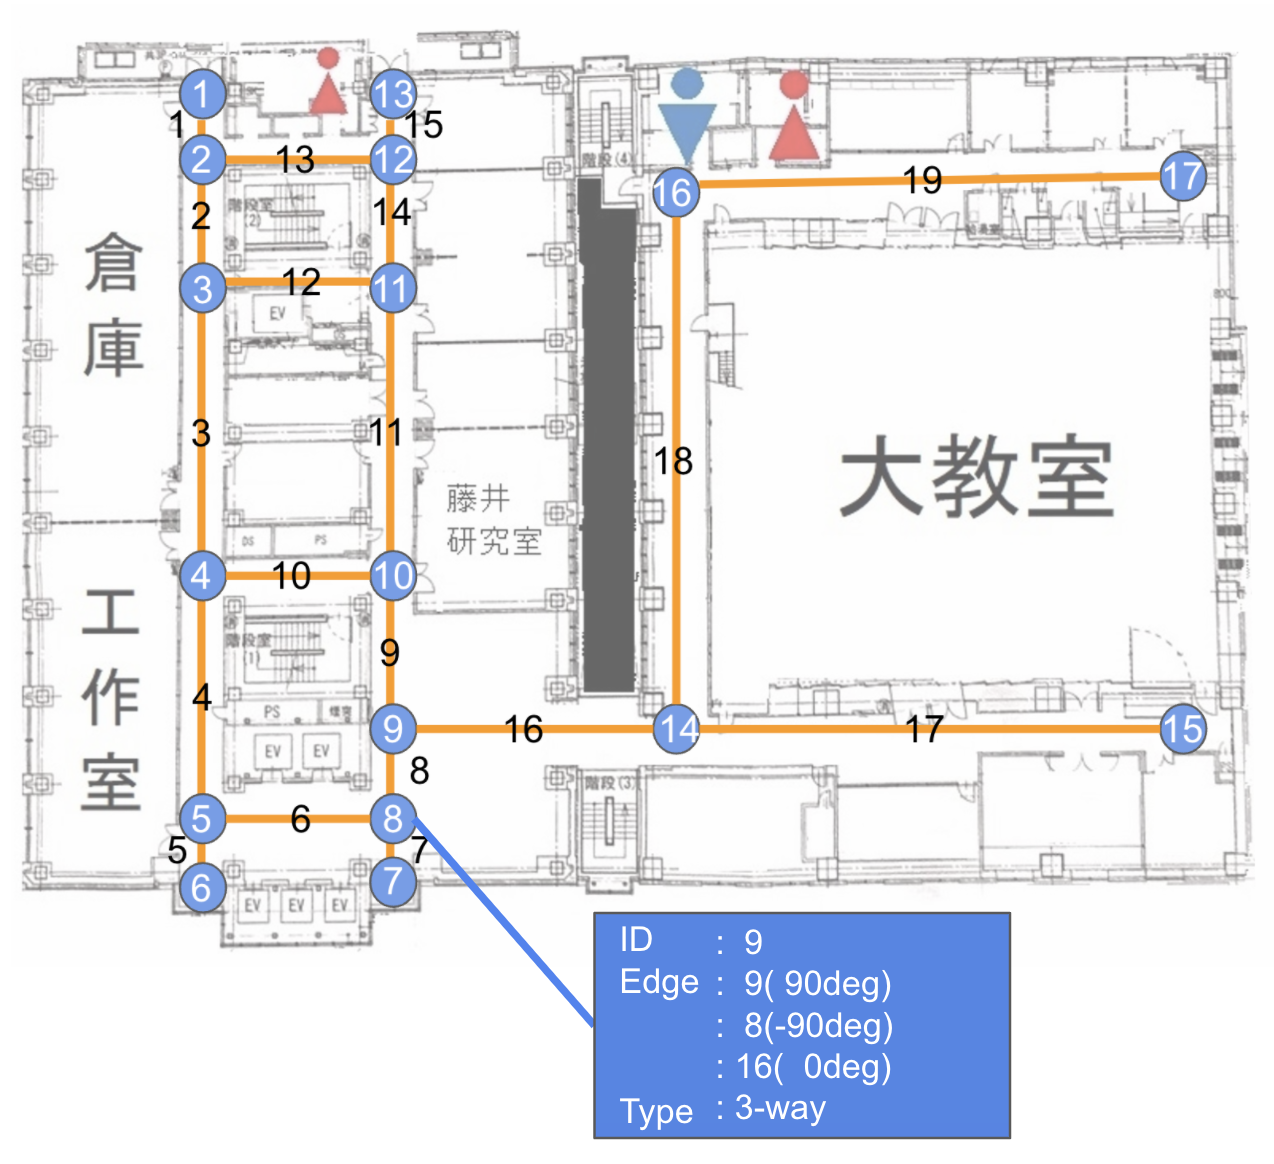
\includegraphics[width = 14cm]{../images/shimada_topological_map.png}
        \caption{Topological map of previous research}
        \label{figure::topologicalmap_simada}
    \end{figure}

    \begin{figure}[H]
        \centering
        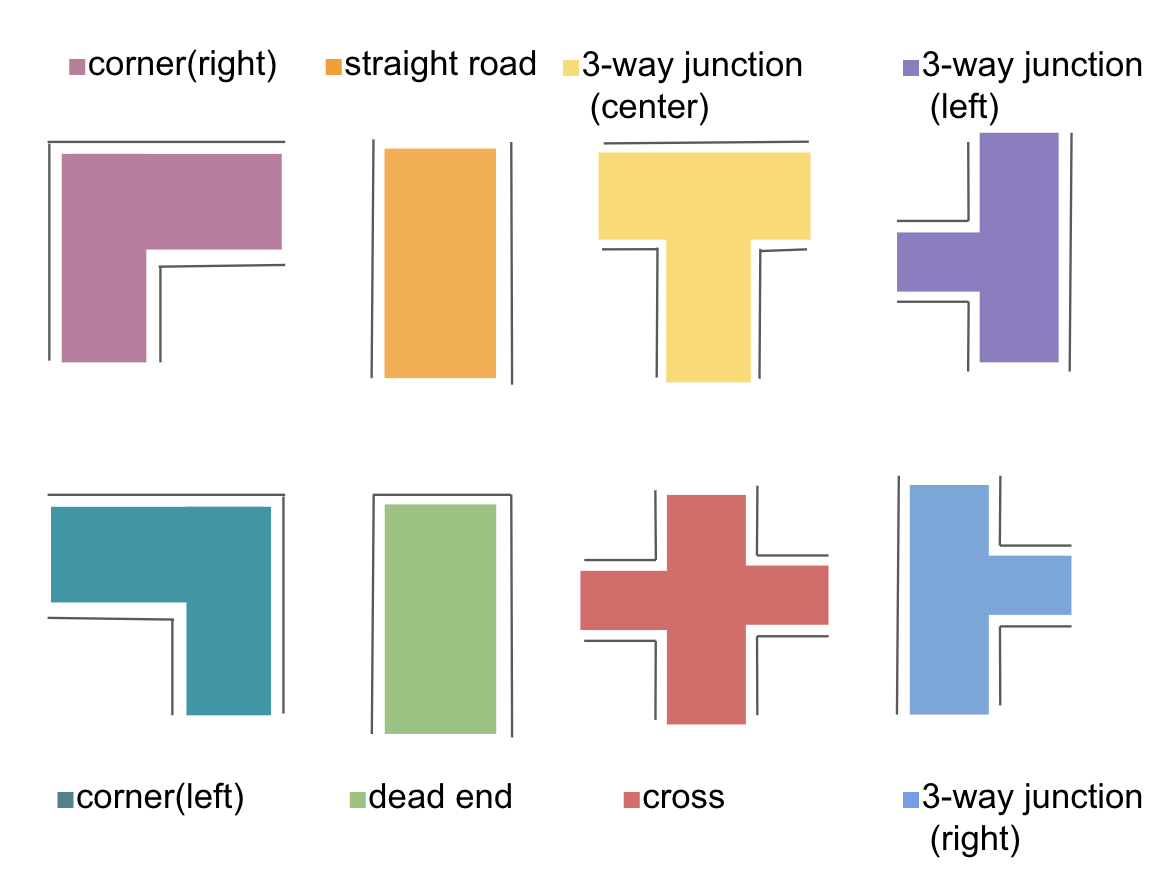
\includegraphics[width = 13cm]{../images/aisle_type2.png}
        \caption{Type of passage}
        \label{figure::aisle_exp}
    \end{figure}

\end{document}